\documentclass[12pt]{article}
\usepackage{fancyhdr}
\usepackage{enumerate,amsmath,graphicx,wrapfig,amssymb,latexsym,amsfonts}
%%%%%%%%%%%%%%           DEFINITIONS, ETC      %%%%%%%%%%%%%%%%%%%%
\newcommand{\lap}{\bigtriangleup}
\newcommand{\C}{\mathcal C}
\renewcommand{\S} {\mathcal S}
\newcommand{\p}{\partial}
\newcommand{\e}{\varepsilon}
\newcommand{\pderiv}[2]{\frac{\partial #1}{\partial #2}}
\def\t{{\bf t}}
\def\u{{\bf u}}
\def\x{{\bf x}}
\def\n{{\bf n}}
\def\stress{{\mathbf{\Sigma}}}
\def\bR{{\bf R}}
\def\npan{n_{\mbox{\tiny{pan}}}}
\def\npt{n_{\mbox{\tiny{pt}}}}
\def\xibar{{\overline{\xi}}}
\def\ombar{{\overline{\omega}}}
\def\abar{{\overline{a}}}
\def\tbar{{\overline{\tau}}}
\def\zbar{{\overline{z}}}
\def\zetabar{{\overline{\zeta}}}
\def\nbar{{\overline{n}}}
\def\ddnb{{\frac{\partial}{\partial \nu}}}%
\def\ddn1{{\frac{\partial}{\partial \nu_Q}}}%
\def\ddnx{{\frac{\partial}{\partial \nu_{Q^k_j}}}}%
\def\ddnq0{{\frac{\partial}{\partial \nu_{Q_0}}}}
\def\mut{{\tilde \mu}}
\def\Ut{{\tilde U}}
\def\Vt{{\tilde V}}
\def\re{{\rm Re}}
\def\im{{\rm Im}}
\def\salph{{s_{\alpha}}}
\def\zalph{{z_{\alpha}}}
%\def\Re{\mbox{Re}}
\def\Re{Re}
\def\om{\omega}
\def\eps{\epsilon}
\def\rhovec{\vec \rho}
\def\y{{\bf y}}
\def\f{{\bf f}}
\def\pfrac#1#2{\frac{\partial #1}{\partial #2}}
\def\remark{\noindent{\bf Remark:}$\quad$}
\newcommand{\eqr}[1]{~(\ref{#1})}
%%%%%%%%%%%%%%%%%%
\begin{document}
\title{Notes for Explicit Kernel-Split Panel-Based Nystr\" om Scheme for Yukawa Boundary Value Problems}
\date{}
\maketitle
\section{Preliminaries}
Consider the following boundary value problem in a simply-connected, bounded domain $\Omega \subset \mathbb{R}^2$:
\begin{eqnarray}
  u(x) - \alpha^2 \Delta u(x) = 0, && {x} \in \Omega,  \nonumber \\
  \lim_{\Omega \ni x' \rightarrow x} u(x') = f(x), && x \in \Gamma,
  \label{dirichlet:bc}
\end{eqnarray}
where $\Gamma$ is the boundary of $\Omega$ and is assumed to be smooth.
We seek the solution $u(x)$ in the form of a double layer potential, 
\begin{equation}
  u(x)=\frac{1}{2\pi\alpha^2}\int_{\Gamma}\pderiv{}{n'}K_{0}
  \left(\frac{|x'-x|}{\alpha} \right) \sigma(x') \, ds', \qquad x \in \Omega, 
  \label{eq:u_dirichlet}
\end{equation}
where $\sigma(x')$ is the value of the unknown
density at the boundary point $x'$, and $\partial / \partial n'$
represents the outward normal derivative at the point $x'$.
Substituting\eqr{eq:u_dirichlet} into\eqr{dirichlet:bc}, we obtain an integral equation for the layer density $\sigma$:
\begin{equation}
  \label{dirichlet:inteqn}
\sigma(x)- \frac{1}{\pi}
  \int_{\Gamma}\pderiv{}{n'}K_{0}\left(\frac{|x' - x|}{\alpha}\right)
  \sigma(x')\, ds' = -2 \alpha^2 f(x) .
\end{equation}

Let $M(x, x')$ be the kernel of the double layer potential, 
\begin{align}
M(x, x') & = -\frac{1}{\pi} \pderiv{}{n'}K_{0}\left(\frac{|x' - x|}{\alpha}\right) \nonumber \\
            & = \frac{1}{\pi \alpha} K_1 \left( \frac{|x' - x|}{\alpha} \right)
                         \frac{x'-x }{|x' - x|} \cdot n' . \label{kernel}
\end{align}
Following the notation of \cite{HelsingHolst}, we will use the subscript $\Gamma$ or $\Omega$ if $x\in \Gamma$ or $x\in \Omega$, respectively.
Hence, 
\begin{align}
\sigma(x) & + \int_\Gamma M_\Gamma(x, x') \sigma(x') ds' = -2 \alpha^2 f(x), \; \; x \in \Gamma \label{IE} \\
u(x) & = -\frac{1}{2\alpha^2} \int_\Gamma M_\Omega(x, x') \sigma(x') ds', \; \; x \in \Omega. \label{DLP}
\end{align}

Consider an $\npt$-point panel-based Nystr\"om discretization scheme based on Gaussian quadrature (see section 3 of \cite{HelsingHolst}). Let $t_i$ and $w_i$, $i = 1, \cdots \, \npan \npt$ be the actual nodes and weights, respectively, on the panels of $\Gamma$ found from transforming the canonical weights and nodes. $M(x,x')$ is not smooth and, as in the case of the Helmholtz equation considered in \cite{HelsingHolst}, can contain both logarithmic- and Cauchy-type singularities, depending on how $x'$ approaches $x$. Special-purpose quadrature is applied to those panels where $M(x,x')$ is not smooth. Introducing the speed function $s(t) = |dx(t)/dt|$, the discretization of\eqr{IE} and\eqr{DLP} is
\begin{align}
\sigma_i + \sum_{j\in{\cal C}(x_i) } M_\Gamma(x_i, x_j) \sigma_j s_j w_{ij}
     + \sum_{j\in{\cal F}(x_i) } M_\Gamma(x_i, x_j) \sigma_j s_j w_{j} = -2 \alpha^2 f_i,  \label{discIE}\\
 u(x) = -\frac{1}{2\alpha^2} \sum_{j\in{\cal C}(x) } M_\Omega(x, x_j) \sigma_j s_j w_{ij}
           -\frac{1}{2\alpha^2} \sum_{j\in{\cal F}(x) } M_\Omega(x, x_j) \sigma_j s_j w_{j}, \label{discDM}
\end{align}
where ${\cal C}(x)$ is the set of source points on panels close to $x$, where special-purpose quadrature weights $w_{ij}$ are used and ${\cal F}(x)$ are the remaining source points.  

\section{Special-Purpose Quadrature}
Now consider the discretization of the integral
\begin{equation}
I_p(x) = \int_{\Gamma_p} G(x, x') \sigma(x') ds', 
\end{equation}
where $\Gamma_p$ is a panel on $\Gamma$, $G(x, x')$ is non-smooth, and the target point $x$ lies close to, or on, $\Gamma_p$. 
Here, if $x\in \Gamma$ then $I_p(x)$ comes from the discretization of\eqr{IE}, and $G(x, x') = M_\Gamma(x, x')$. 
If $x\in\Omega$, we are considering the discretization of\eqr{DLP}, and $G(x, x') = -M_\Omega(x, x')/2 \alpha^2$.

\subsection{Logarithmic singularity plus smooth part} 

If $x\in \Gamma$, $G(x, x')$ can be expressed as 
\begin{equation}
G(x, x') = G_0(x, x') + \log|x - x'| G_L(x, x'). \label{Gon}
\end{equation}
The special quadrature to compute $I(x_i)$, where the target point $x_i$ on $\Gamma_p$, is described by equation (30) in \cite{HelsingHolst}.  To use this formula, we need $G_0(x_i, x_i)$ and $G_L(x_i, x_j)$, which is found by considering the singularity structure of\eqr{kernel}. 
According to NIST's DLMF (see http://dlmf.nist.gov/10.31)
\[
K_1(z)  = \frac{1}{z} + \ln \left( \frac{1}{2} z \right) I_1(z) + \tilde K_1(z),
\]
where $I_1(z)$ is the modified Bessel function of the first kind  of order 1 and $\tilde K_1(z)$ is a smooth function in $z$. As $z\rightarrow 0$, both of these functions have a  limit of zero. 
This gives
\begin{equation}
G_L(x_i, x_j)  = \frac{1}{\pi \alpha} I_1\left(\frac{|x_j - x_i |}{\alpha} \right)\frac{x_j - x_i }{|x_j - x_i|} \cdot n_j.
\label{GL}
\end{equation}
and
\begin{align*}
G_0(x_i, x_i) & = \lim_{x_j \rightarrow x_i} G(x_i, x_j) \\
                     &  = - \frac{1}{2\pi} \frac{ n_i \cdot \ddot{x}_i }{|\dot{x}_i|^2 }, 
\end{align*}
where $\dot{x} = dx(t)/dt$, and $\ddot{x} = d^2 x(t)/ dt^2$. An alternative expression to the above is $G_0(x_i, x_i) = \kappa_i/ 2 \pi$, where $\kappa$ is the curvature.

\noindent
\textsc{A note about the code:} The MATLAB routine \texttt{dlpYukawaPanelMatrix} returns the system matrix associated with the left-hand side of\eqr{IE}, including the modifications made here for product integration for singular integrals. It is implemented exactly as described in \cite{HelsingHolst}, and includes the use of the MATLAB function \texttt{WfrakLinit} described in Appendix A of that paper. 


\subsection{Logarithmic and Cauchy-type singularities plus smooth part} 
If $x\in\Omega$, $G(x, x')$ is written as 
\begin{equation}
G(x, x') = G_0(x, x') + \log|x - x'| G_L(x, x') + \frac{(x' - x) \cdot n' }{|x' - x|^2} G_C(x, x'), \label{G}
\end{equation}
where $G_0(x, x')$, $G_L(x, x')$ and $G_C(x, x')$ are smooth functions. 
Here, $G_L(x, x')$ is the same as\eqr{GL} except scaled by $-1/2 \alpha^2$, and
\[
G_C(x, x') = -\frac{1}{2\pi \alpha^2}.
\]

The special quadrature to compute $I_p(x)$, where $x\in \Omega$ and close to $\Gamma_p$ is calculated according to equation (33) in \cite{HelsingHolst}. The compensated weights $w_{Lj}^{\mbox{corr}} (x)$ and $w_{Cj}^{\mbox{corr}} (x)$ are computed with the MATLAB function \texttt{wLCinit} found in Appendix $B$ in \cite{HelsingHolst}, taking into account the change in orientation of the point $x$ with respect to $\Gamma_p$. In \cite{HelsingHolst}, $x \in \Omega^c$, i.e. in the unbounded domain exterior to $\Gamma$. This requires a change in how $p_1$ is calculated (see section 7 of \cite{HelsingOjala}). The following modification is included in  \texttt{wLCinit}: \\
\texttt{
\noindent if imag(rtr) < 0 \&\& abs(real(rtr)) < 1 \\
 \hspace{.5in} p(1) = p(1) + 2*1i*pi; \\
 \hspace{.5in}         p1 = p1 - 2*1i*pi;  \\
    end. \\
}

\noindent \textsc{A note about the code:} The MATLAB routine \texttt{dlpYukawaPanelNSEval} evaluates\eqr{DLP} when $x$ is close to the source curve $\Gamma$. If $x$ is not close, the routine  \texttt{dlpYukawaPanelEval} does this evaluation.



\section{Example}
The following example was calculated using the routine \texttt{ModHelmPanelDriver}. 
The boundary value problem\eqr{dirichlet:bc} is solved with boundary conditions prescribed by the exact solution
\[
u(x) = K_0 \left( \frac{|z - z^*|}{\alpha} \right) 
\]
on the star-shaped domain shown in the figure below. The boundary is  discretized with 100 panels using 16-point quadrature. The integral equation\eqr{discIE} is solved directly in MATLAB.  A 200x200 grid is superimposed over the domain, resulting in 24258 interior points. In this case, the minimum source-to-target distance is $2.6 \times 10^{-4}$. In this grid, \eqr{discDM} is evaluated. The largest point-wise error on the grid is $1.1 \times 10^{-14}$.  At a set of target points well-separated from the boundary, the largest point-wise error is $2.1 \times 10^{-16}$.

\begin{center}
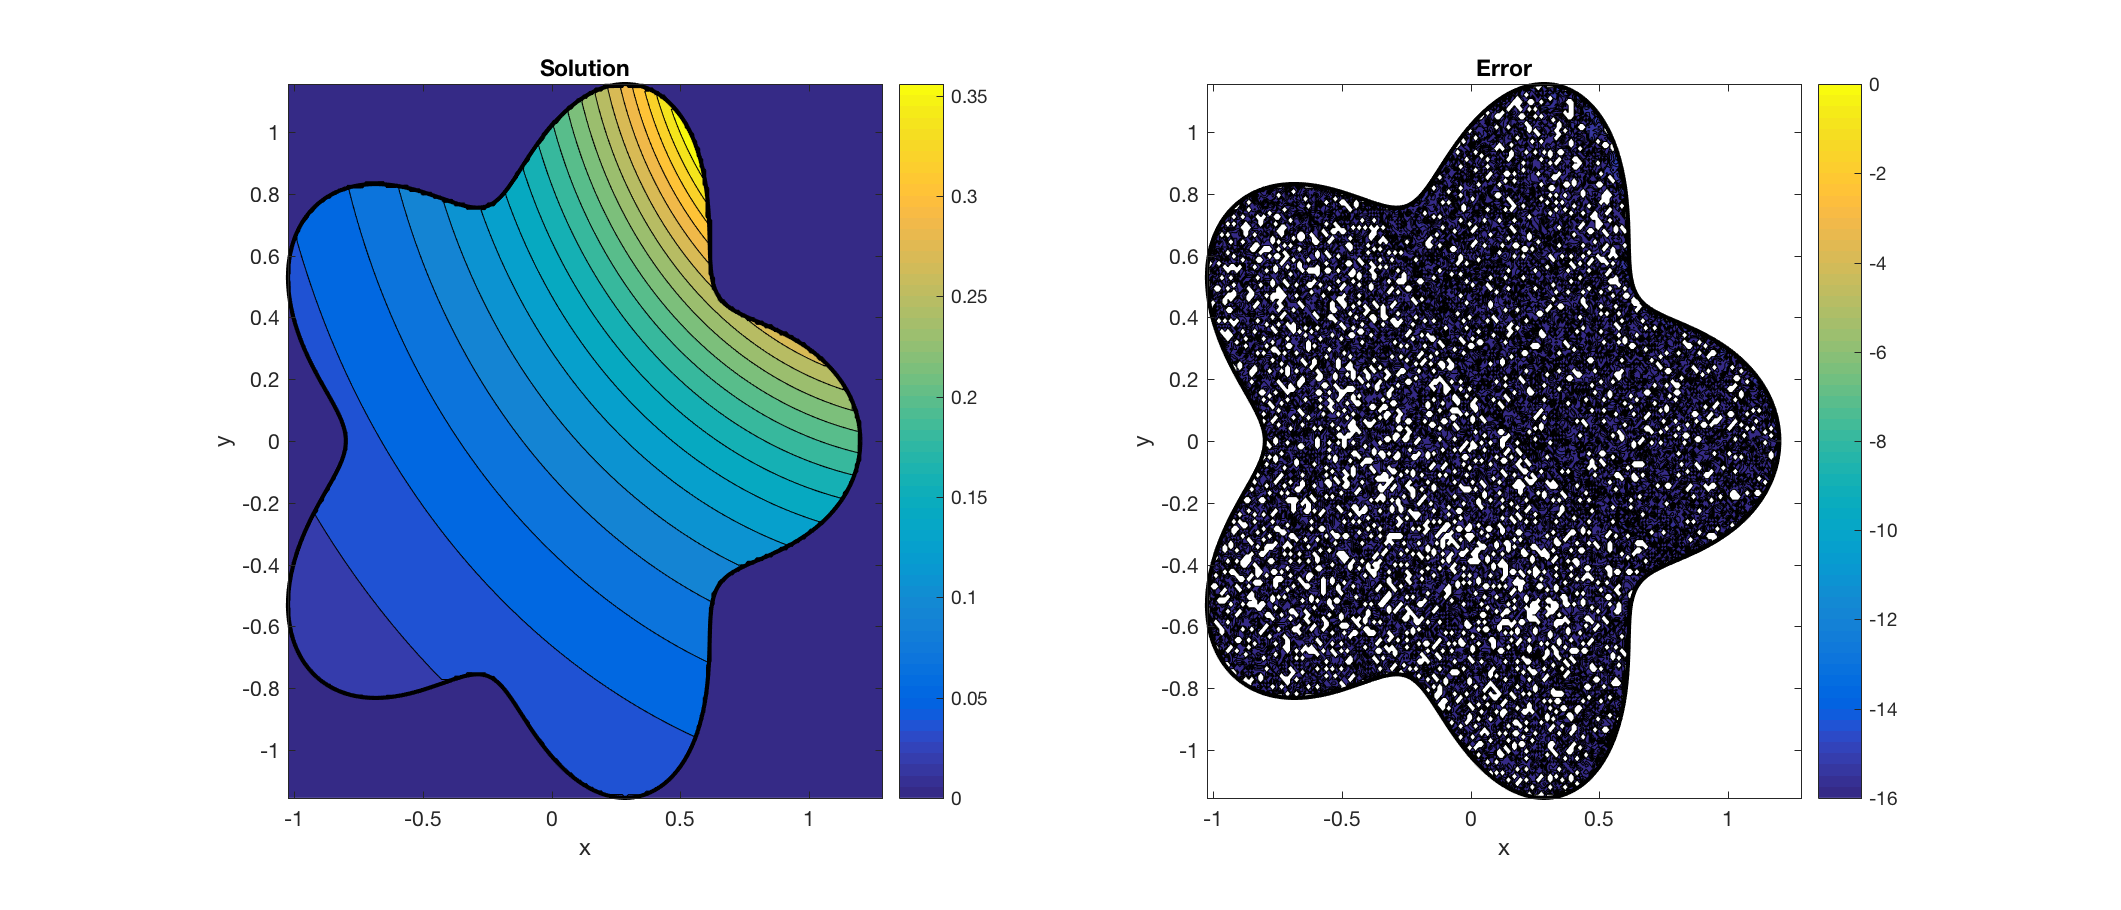
\includegraphics[width=6in]{Yukawa_Ex.eps}
\end{center}

\noindent \textsc{Further Comments about Implementation:} In section 8 of \cite{HelsingHolst}, four schemes are proposed which use the approach to quadrature described above. We have implemented scheme A, the approach described here, only. While the most straightforward, it shows the poorest convergence for the Helmholtz Equation.  It may be worthwhile implementing one of the other experiences, however scheme A already achieves significantly superior results to the Alpert quadrature rules at points well-separated from source points (by about 3 orders of magnitude) \cite{KropinskiQuaife} and QBX for close-evaluation. 


\begin{thebibliography}{10}

\bibitem{HelsingHolst}
J.~Helsing and A.~Holst.
\newblock Variants of an explicit kernel-split panel-based Nystr\" om discretization scheme for Helmholtz boundary value problems.
\newblock {\em Adv. Comput. Math}, 41:691--708, 2015.

\bibitem{HelsingOjala}
J.~Helsing and R.~Ojala.
\newblock On the evaluation of layer potentials close to their sources.
\newblock {\em J. Comp. Phys.}, 227:2899--2921, 2008.

\bibitem{KropinskiQuaife}
M.C.A. Kropinski and B.D. Quaife.
\newblock Fast integral equation methods for the modified Helmholtz equation.
\newblock {\em J. Comp. Phys.}, 230:425--434.

\end{thebibliography}
\end{document}